\subsection{Architektur}

Der systematische Aufbau des Volksbots ist in Abbildung \ref{fig:architecture_volksbot} dargestellt. Die Funktionen des Roboters basieren auf der Auswertung und Ansteuerung der Sensoren bzw. Aktoren. Alle Operationen, wie z.B. die Lokalisation, die Routenplanung, der Vorgang der Paketübergabe, laufen auf dem Robot Operating System und nutzen die Daten der Sensorik zur geeigneten Ansteuerung der Aktoren. Gesteuert werden die Operationen über die externe Kommunikationsebene, welche aus einem MICAz-Modul besteht. Hier werden Aufträge empfangen und auf der Operationsebene in zugehörige Ziele übersetzt.

\begin{figure}[h!]
 \centering
		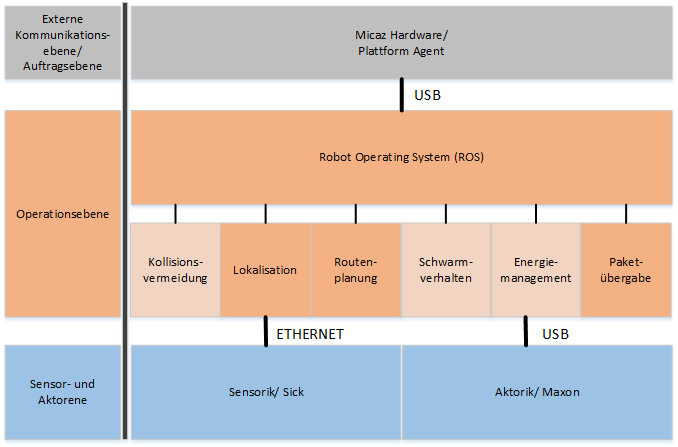
\includegraphics[width=1\textwidth]{drive/DRIVE_Architektur.png}
	\caption{Architektur des Volksbot}
	\label{fig:architecture_volksbot}
\end{figure}

Die in dunkleren rot hervorgehobenen Funktionen der Operationsebene deuten deren höhere Wichtigkeit an und geben ein erstes Anzeichen darauf welche Funktionen erfolgreich umgesetzt werden konnten.